\section{Sistema a lazo abierto}

En esta sección se realiza el análisis del sistema a tratar, en particular, se trataran las ecuaciones de estado  y función transferencia a lazo abierto. En vista a ello, en primer lugar, se presenta la topología de estudio:

\begin{figure}[H]
  \centering
  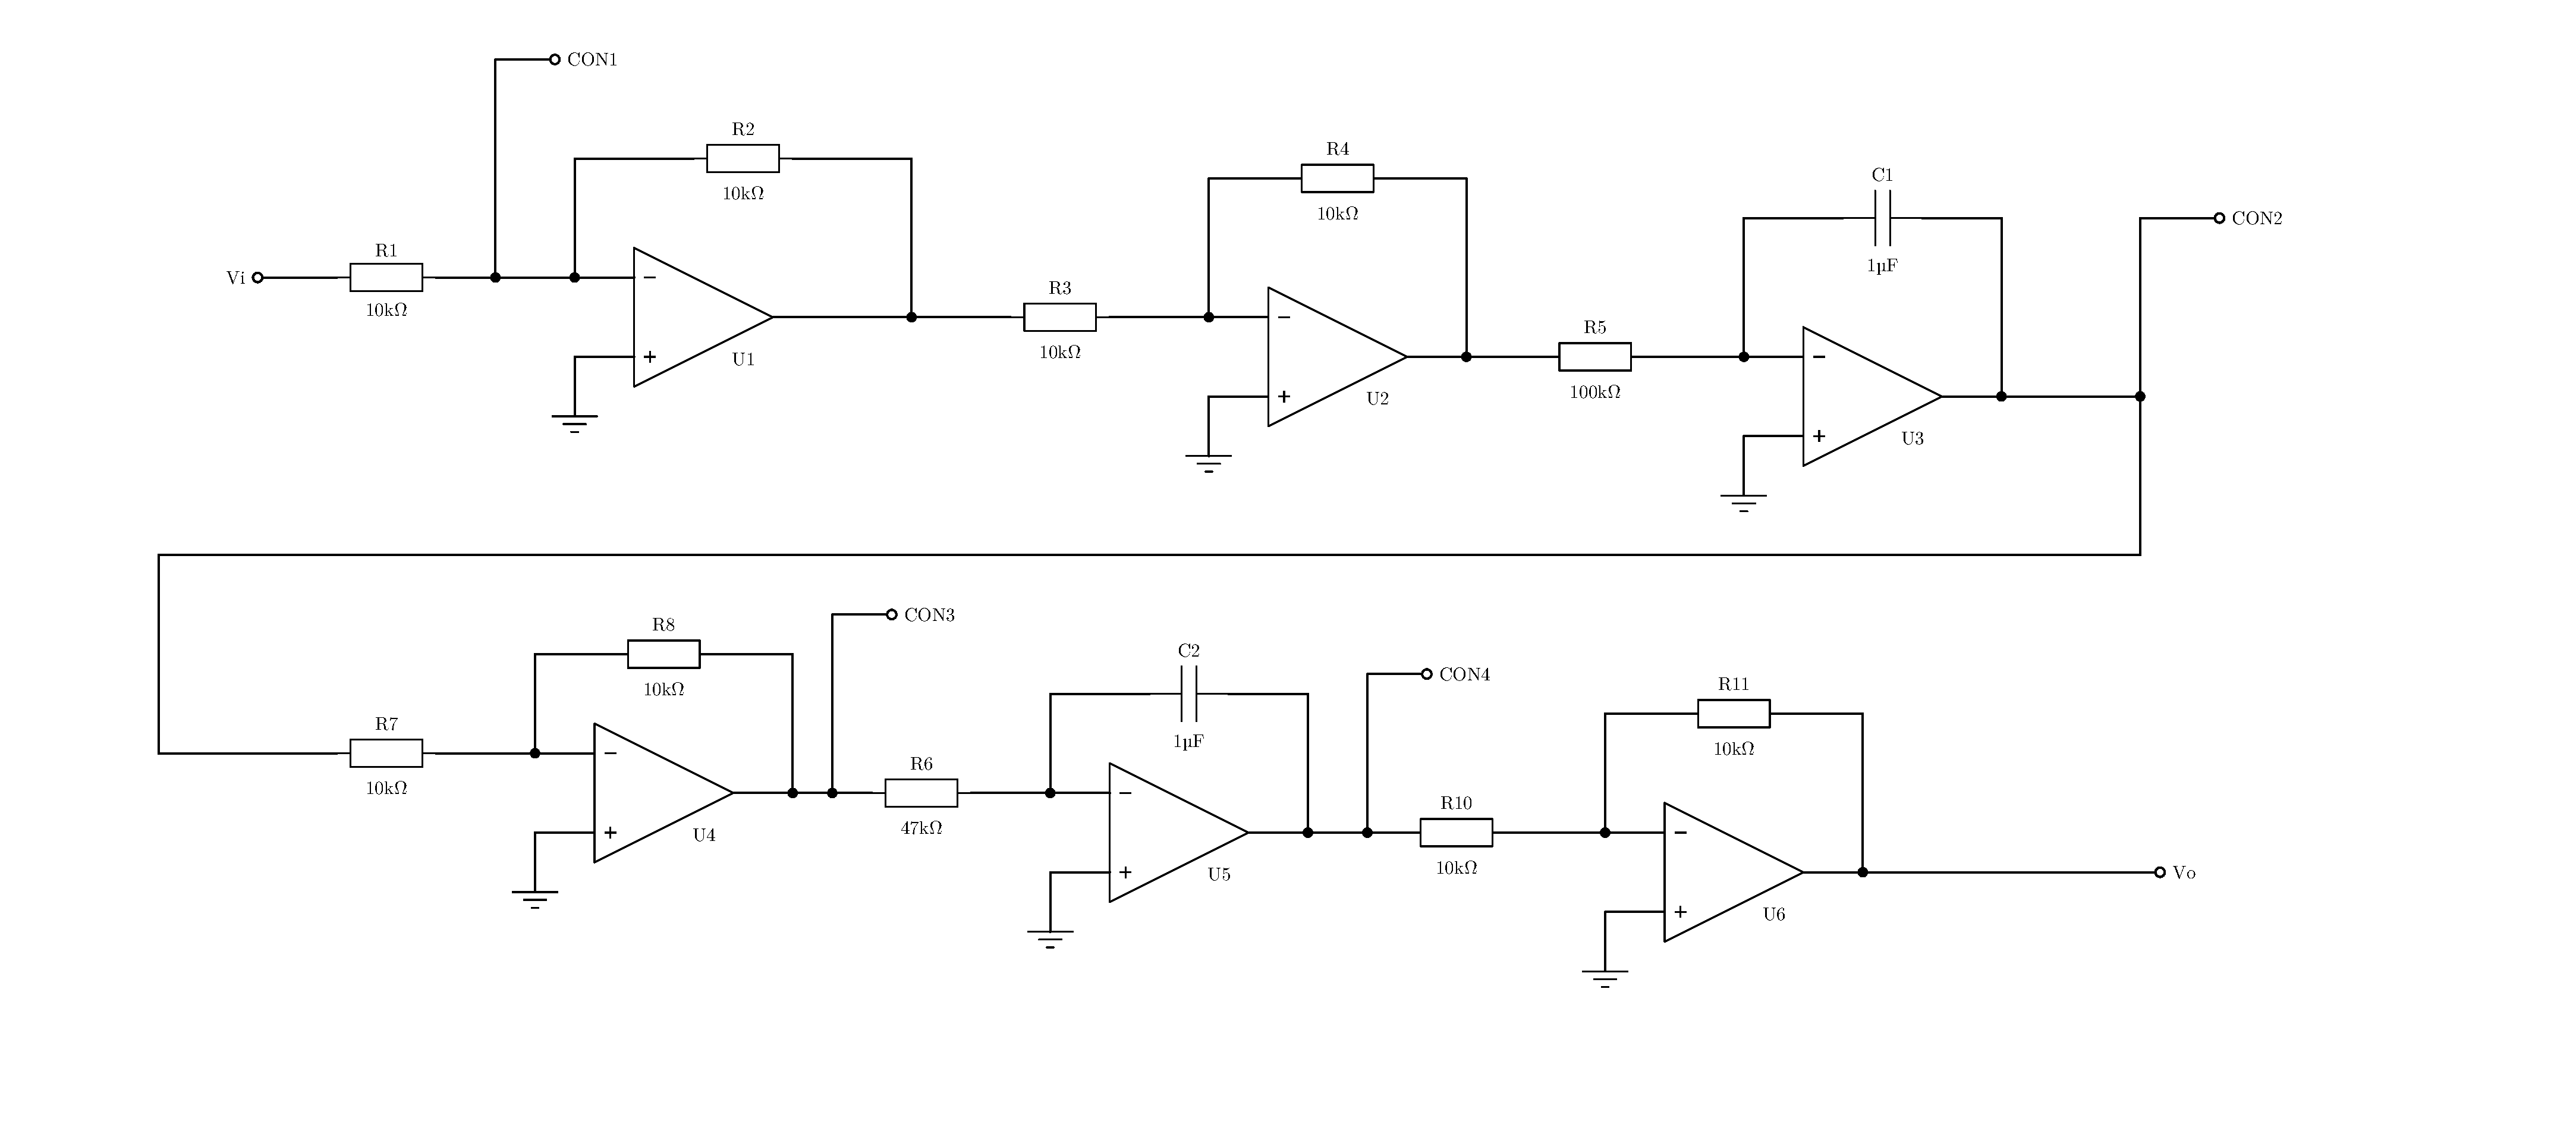
\includegraphics[width = \textwidth]{Imagenes/2_Analisis_lazo_abierto/representacion.pdf}
  \caption{Sistema a lazo abierto | Circuito.}
  \label{fig: sistema a lazo abierto}
\end{figure}


\noindent Esta configuración se puede representar bajo el siguiente diagrama en bloques en cascada:

\vspace{1cm}
\begin{figure}[H]
  \centering
  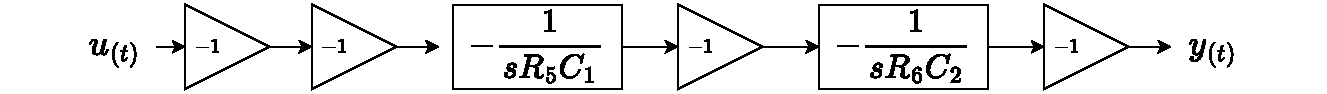
\includegraphics[width = \textwidth]{Imagenes/2_Analisis_lazo_abierto/Lazo abierto.drawio (1).pdf}
  \caption{Sistema a lazo abierto | Diagrama en bloques.}
  \label{fig: sistema a lazo abierto diagrama}
\end{figure}

\noindent por lo que se obtiene la transferencia a lazo abierto:

\begin{equation}
    G_{(s)} = \frac{Y_{(s)}}{U_{(s)}} = \frac{1}{s^2 \cdot R_5 \cdot C_1 \cdot R_6 \cdot C_2} = \frac{G_0}{s^2} = \frac{10 \cdot 21.277}{s^2}
\end{equation}

\noindent donde se omitieron las unidades del numerador por simplicidad. En función de esta ecuación es posible reescribir la ecuación de estado correspondiente. En vista a ello se despeja convenientemente:

\begin{align*}
    Y_{(s)} \cdot s^2 = G_0 \cdot U_{(s)}
\end{align*}

\noindent anti-transformando miembro a miembro:

\begin{align*}
    \ddot{y}_{(t)}= G_0 \dot u_{(t)}
\end{align*}

\noindent Definiendo las siguientes variables de estado:

\begin{align*}
\begin{cases}
    x_1 = y\\
    x_2 = \dot{x_1}
\end{cases}
\end{align*}

\noindent de este modo:

\begin{align*}
\begin{cases}
    \dot{x_1} = \dot{y}\\
    \dot{x_2} = \ddot{x_1} = \ddot{y}
\end{cases}
\end{align*}

\noindent por ende la ecuación diferencial asociada puede reescribirse en función de las variables de estado como:

\begin{equation}
\begin{cases}
    \dot{x_2} = G_0 \cdot u\\
    y = x_1
\end{cases}
\end{equation}

\noindent de manera matricial: 


\begin{equation}
\begin{aligned}
\dot{\mathbf{x}} &=
\underbrace{
\begin{bmatrix}
0 & 1 \\
0 & 0
\end{bmatrix}
}_{A}
\mathbf{x}
+
\underbrace{
\begin{bmatrix}
0 \\
G_0
\end{bmatrix}
}_{B}
[u] \\
[y] &=
\underbrace{
\begin{bmatrix}
1 & 0
\end{bmatrix}
}_{C}
\mathbf{x}
+
\underbrace{[0]}_{D} \, [u]
\end{aligned}
\end{equation}